\documentclass[tikz,border=14pt]{standalone}
\usepackage{amsmath,amssymb}
\usetikzlibrary{arrows.meta}
\definecolor{ink}{HTML}{E4EDF8}
\definecolor{muted}{HTML}{596B80}
\definecolor{blue}{HTML}{9FC2FF}
\definecolor{teal}{HTML}{63D3BB}
\definecolor{gold}{HTML}{E7C274}
\definecolor{panel}{HTML}{111923}
\pagecolor{panel}
\color{ink}
\begin{document}
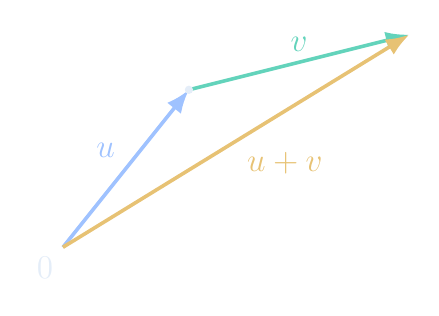
\begin{tikzpicture}[font=\large,text=ink,vec/.style={-{Latex[length=3mm]},line width=1.3pt},axis/.style={muted,-{Latex[length=2mm]},thin}]
\coordinate (O) at (0,0);\coordinate (A) at (1.6,2);\coordinate (B) at (4.4,2.7);
\draw[vec,blue] (O)--(A) node[midway,above left] {$u$};
\draw[vec,teal] (A)--(B) node[midway,above] {$v$};
\draw[vec,gold] (O)--(B) node[midway,below right] {$u+v$};
\node[below left] at (O) {$0$};
\fill[ink] (A) circle (1.5pt);
\end{tikzpicture}
\end{document}
